\documentclass[a4paper,twoside]{article}

\usepackage{epsfig}
\usepackage{subfigure}
\usepackage{calc}
\usepackage{amssymb}
\usepackage{amstext}
\usepackage{amsmath}
\usepackage{amsthm}
\usepackage{multicol}
\usepackage{pslatex}
\usepackage{apalike}
\usepackage{SCITEPRESS}
\usepackage[small]{caption}
\usepackage{url}

\subfigtopskip=0pt
\subfigcapskip=0pt
\subfigbottomskip=0pt

\begin{document}

\title{SuperPhy: A Resource for Integrated Phylogenetic and Epidemiological Analysis of Pathogens}

\author{\authorname{Matthew D. Whiteside\sup{1}, Chad Laing\sup{1}, Akiff Manji\sup{1} and Victor P.J. Gannon\sup{1}}
\affiliation{\sup{1} Laboratory for Foodborne Zoonoses, Public Health Agency of Canada, Lethbridge, AB, Canada Canada}
\email{{mawhites, chad.r.laing, ??akiff??, vic.gannon}@phac-aspc.gov.ca}}

\keywords{Population Genomics, Epidemiology, Phylogeny, Bacterial Pathogenesis}

\abstract{The abstract should summarize the contents of the paper and should contain at least 70 and at most 200 words. The text must be set to 9-point font size.}

\onecolumn \maketitle \normalsize \vfill

\section{\uppercase{Introduction}}
\label{sec:introduction}

\noindent Centralized massively parallel nucleic acid sequencing has led to an exponential increase in genomic data generation that threatens to outpace advances in data storage and analysis \cite{kahn_future_2011,teeling_current_2012}. In addition, small distributed sequencing platforms such as the IonTorrent and MiSeq have emerged that promise to provide point of care / investigation capabilities with near-real time generation of genomic data \cite{loman_performance_2012}. This capability will allow the research community to rapidly disseminate data, especially where decisions may be time-critical; e.g., in clinical medicine and epidemiological investigations. Better algorithms, more powerful analytical tools and state-of-the art infrastructure are needed to analyze these datasets in near-real time, store the raw and computed data and provide the essential biological information to a wide range of end-users, including those with little or no training in bioinformatics, in readily understandable and useful formats.

Efforts to simplify bioinformatics workflows such as Taverna \cite{lanzen_taverna_2008} and Galaxy \cite{goecks_galaxy:_2010} have been created, and provide an effective means for users to create bioinformatics workflows. However, data is not integrated with these tools, requiring transfer of genomic sequences from public or private databases, the re-computation of analyses and the inability to compare thousands of genomes. Likewise, online repositories of genomic sequence data such as the National Center for Biotechnology Information (\url{http://www.ncbi.nlm.nih.gov/}) and the Genomes Online Database (\url{http://www.genomesonline.org/cgi-bin/GOLD/}) 
provide a wealth of data, but are decoupled from an efficient analysis platform. Additionally, storage and computational analysis of thousands of genomes has moved beyond the standard desktop computer, and even with more memory, efficient methodologies and algorithms, servers storing and analyzing thousands of genomic sequences require leading-edge hardware, and the ability to scale in order to meet the computational requirements projected by this increase in data.

We have previously designed Panseq, a suite of software tools called for the automated comparison of multiple genomes \cite{laing_pan-genome_2010,laing_identification_2011}. Panseq is based on the concept of the bacterial pan-genome, the outputs of which enhance our understanding of the evolution of specific bacterial groups, and the genetic basis of important phenotypic traits which differ among these groups.

By building upon capability of Panseq and integrating it with public genomic data, we hope to transform the way the research community analyzes genomic data. In light of the torrent of sequencing data that has been generated and the uptake of distributed sequencing technologies that can provide near-real time data, we have created a counterpart computational platform, called SuperPhy (\url{http:xxx.xxx.xxx.xxx}), that can provide near-real time analyses. It currently provides all publicly available data for \textit{Escherichia coli}, pre-computed analyses of the data and novel analyses tools that will decrease computation times and will allow rapid assessment of user-uploaded data. The web-interface to this computational platform obviates the need for command-line skills, or a particular computer environment. As more of the research community uses the platform, the number of genomic sequences it has processed / analyzed will increase, adding further value to the platform and thus will attract more users. The SuperPhy platform provides data outputs that serve a wide community of users, with translation of the genomic data into biologically relevant reports, useful to researchers in a variety of disciplines.

\section{\uppercase{Design}}
\label{sec:design}

\noindent SuperPhy is an interactive web platform that integrates public \textit{E. coli} genome data with meta-genomic analysis tools.  Users can also upload their own genome sequences for analysis.  The platform is designed to be flexible and can work with finished genomes or genomic contigs from the assembly stage. 

\subsection{Database Schema}

The current focus of the SuperPhy platform is on analyzing \textit{E.coli}, however, the SuperPhy database was designed from the start to be extensible to other species. To make the database flexible, we chose to use the Chado relational schema \cite{mungall2007chado}. Chado was originally developed for storing model organism genomic data, but because of the central role of ontologies in Chado, it is also suited to storing meta-genomic data needed for phylogenetic and epidemiological analyses. In Chado, ontologies are used to assign types to entities, attributes and relationships \cite{mungall2007chado}. This ontology-centric design makes Chado highly adaptable. By not defining types in relational layer and instead using a mutable controlled vocabulary to assign types, the schema can be easily re-used or changed over time without having to change the relational structure \cite{mungall2007chado}.  Figure \ref{fig:ontology} shows the main entity types and corresponding relationship types used in our SuperPhy instance of the Chado schema (not shown are the attributes such as sequence locations or  meta-data). \texttt{Contig Collection} is the parent term assigned to any complete or incomplete genome project uploaded by a user or obtained from an external database.  It does not directly contain any sequence data; it is used to store global attributes for a genome. A \texttt{Contig Collection} will be linked to one or more DNA sequences that we label \texttt{Contig}. The \texttt{Contig} types can be assembled contigs or fully sequenced chromosomes or plasmids (molecular type is distinguished at the attribute level). \texttt{Contig} and \texttt{Contig Collection} make up the supplied genome data. Further experimental features are calculated and added for each genome. The presence of Pan-genome loci in the individual isolate genomes is recorded using the \texttt{Locus} type. SNPs are calculated and recorded in the conserved core genome regions. Alleles of known virulence factor and antimicrobial resistance genes are identified and recorded with the allele type.  A more detailed description of the pipeline for identifying SNPs, loci and alleles is provided in section \ref{sec:pipeline}.

\begin{figure*}[t]
  \vspace{-0.2cm}
  \centering
   {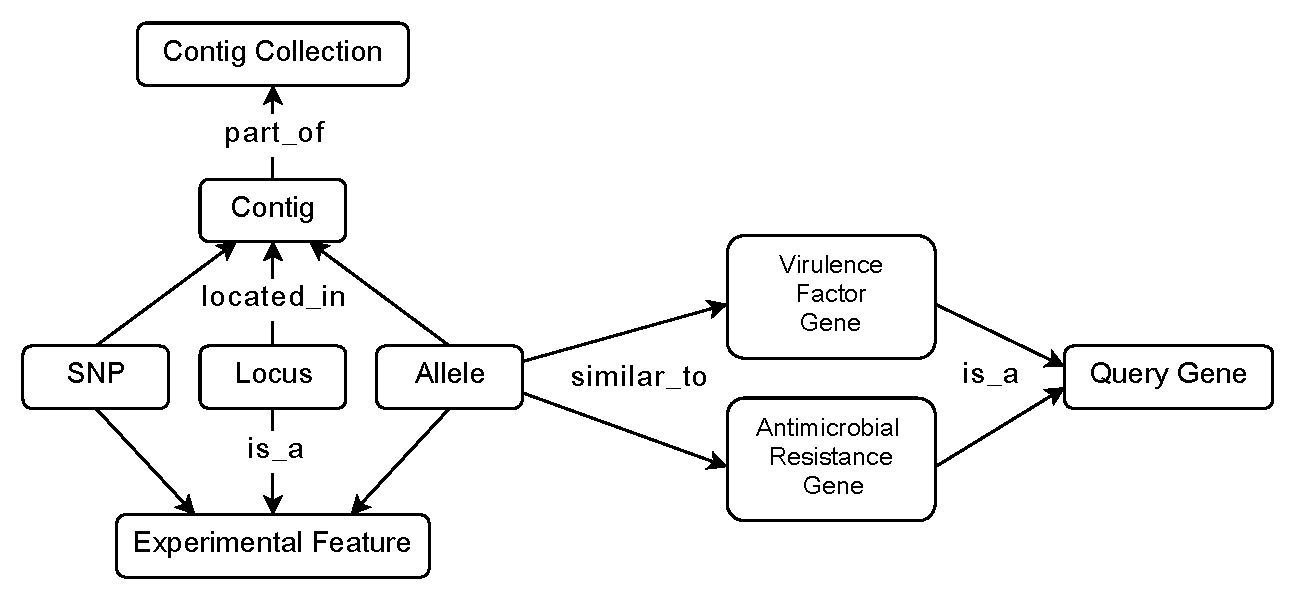
\epsfig{file = ontology.eps, width = 12cm}}
  \caption{A ontology graph representing the main feature types used in the SuperPhy schema.}
  \label{fig:ontology}
  %\vspace{-0.1cm}
\end{figure*}

\subsection{Analysis Pipeline}
\label{sec:pipeline}

The tool PanSeq supports the SuperPhy platform \cite{laing_pan-genome_2010}. Genome sequences uploaded by users or obtained from NCBI Genbank and Whole Genome Sequence repositories \cite{benson2013genbank} are input into PanSeq to identify segments that belong to the conserved core genome and to the more variable accessory genome. PanSeq works by iteratively aligning genomes using the MUMmer 3 program to produce a non-redundant pan-genome sequence \cite{laing_pan-genome_2010,kurtz2004versatile}. The pan-genome is then compared back to the input genomes to generate a listing of the presence or absence of each genomic loci in the pan-genome across the input genomes. PanSeq also catalogs the SNP variations in the conserved regions \cite{laing_pan-genome_2010}.  The loci and SNPs identified by PanSeq are loaded into the SuperPhy database. ??Annotations for the pan-genome regions are provided by a pre-computed BLASTx analysis.??

A second analysis identifies virulence and drug resistance determinants in the genomes. Starting with a predefined set of query virulence and antimicrobial resistance genes, the PanSeq tool searches for alleles of these genes in the input genomes. PanSeq uses BLASTn to conduct the search. To produce a non-redundant query set of antimicrobial resistance genes, all AMR genes were downloaded from the Comprehensive Antibiotic Resistance Database \cite{mcarthur2012card} and then clustered based on sequence similarity using BLASTclust. Representatives from each cluster were selected first on the basis of the species' phylogenetic distance to \textit{E. coli} and secondly, on the length where longer sequences were selected over shorter ones. All query AMR genes are organized according to their Antimicrobial Resistance Ontology annotation to aid in identifying the presence of different antimicrobial resistance mechanisms. The virulence gene set was produced by obtaining all gene alleles of known virulence factors in \textit{E. coli} from the Virluence Factor Database \cite{chen2012vfdb,chen2005vfdb}.  The longest allele was selected for each VF gene, except in cases where sequence similarity was less than 90\%, in which case, multiple alleles were included the VF query set for a particular gene.

\subsubsection{Constructing and Displaying Phylogenetic Trees}

Global phylogenetic trees, in SuperPhy, are used in the results displays to show the phylogenetic position of a genome and also in the query forms, to allow users to select genomes based on tree location. A maximum-likelihood phylogenetic tree is constructed for all \textit{E. coli} genomes in the database. The tree is built from a multiple sequence alignment of the conserved core genome regions. The tree initially contains all genomes, but is dynamically pruned to show specific genomes. The phylogenetic tree is displayed graphically using the D\sup{3} javascript library \cite{bostock2011d3}. The graphical interface was designed to be interactive; providing the ability to pan, zoom and expand, collapse or select tree nodes.


\subsubsection{Assigning Stx Subtypes}

Not sure if this will be completed in time.

\subsection{Meta-data}

Meta-data is invaluable for the biological interpretation of genome sequence data, but to maximize its usefulness, meta-data must be standardized. We developed in SuperPhy a predefined set of meta-data fields and permissible values. The meta-data types capture the key bacterial isolate attributes that characterize \textit{E. coli} infections. User compliance with these meta-data standards is aided by using context-dependent drop-down fields in the genome upload form. Selecting one of the fields will alter the available options in other fields (for example, selecting \textit{H. sapiens} as the host species will change the isolation sources and disease options that the user can select).  However, we also find it necessary to allow users to optionally define values for certain meta-data types such as the diseases and symptoms associated with an isolate. Table \ref{tab:metadata} shows the meta-data types employed in SuperPhy.

\begin{table*}[t]
\caption{Genome meta-data captured in the SuperPhy database.}
\label{tab:metadata} \centering
\begin{tabular}{|l|c|p{6cm}|}
  \hline
  \textbf{Field} & \textbf{Required} & \textbf{Description} \\
  \hline
  Name &  \checkmark & Genome name\\
  \hline
  Host & \checkmark & Species that was source of isolate \\
  \hline
  Source & \checkmark & Source tissue or material for isolate \\
  \hline
  Serotype & \checkmark & Antigen type designation \\
  \hline
  Strain & \checkmark & Organism subtype \\
  \hline
  Date & \checkmark & Date isolate was obtained \\
  \hline
  Molecular type & \checkmark & Chromosome, plasmid or contig \\
  \hline
  Location &  & Location isolate was obtained from \\
  \hline
  Syndrome &  & Associated diseases or symptoms \\
  \hline
  Age &  & Host age \\
  \hline
  PMID &  & Pubmed IDs of associated articles \\
  \hline
  External ID &  & External DB accessions \\
  \hline
  Description &  & Genome description \\
  \hline
  Comments &  & Free-form comments by submitter  \\
  \hline
  Keywords &  & General keywords to characterize genome\\
  \hline
  Finished &  & Indicates complete genome sequence \\
  \hline
  Owner &  & Source laboratory \\
  \hline
\end{tabular}
\end{table*}


\section{\uppercase{Functionality}}
\label{sec:functionality}

\subsection{Uploading a Genome}

Users can upload their \textit{E. coli} genomes to SuperPhy for analysis and comparison to the database's other \textit{E. coli} genomes.  Access to uploaded genomes is regulated by the user. Users can select to keep their genome data private indefinitely, immediately make it publicly viewable, or choose to release it after a specified date.  While private, users can grant other users access to their genomes.  Access is defined by three roles: view only, modify (additionally allows users to change meta-data) and admin (provides full privileges to modify, delete or grant additional access to the genome).

\subsection{Retrieving Genome Meta-data}

Existing \textit{E. coli} genomes from the NCBI Genbank and Whole Genome Sequence repositories \cite{benson2013genbank} have been loaded into the SuperPhy database. Meta-data in these sources were mapped to our standardized set of meta-data types and values (see Table \ref{tab:metadata}). To facilitate navigation,
users can choose to display one or more of several types of meta-data in the forms (host species, isolation source, isolate date can be displayed alongside genome name). Through the advanced search facility, genome information can be queried by selecting from a interactive phylogenetic tree, from a world map, by date range or by boolean search of user-defined search fields and keywords.  The sophisticated query interface is designed to address a broad range of hypotheses based on meta-data or phylogenetic information (Figure \ref{fig:search}).

\begin{figure*}[t]
  \vspace{-0.2cm}
  \centering
   {
\epsfig{file = superphy_forms.eps, width = 16cm}}
  \caption{Advanced search function in SuperPhy. Genome information can be queried by (A) interactive phylogenetic tree (B) world map or (C) boolean search of user-specified fields and keywords. }
  \label{fig:search}
  %\vspace{-0.1cm}
\end{figure*}

\subsection{Groupwise Comparisons of the Distribution of SNPs and Loci}

The \textit{E. coli} pan-genome is highly variable. To help correlate phenotype and genotype, SuperPhy provides the ability to compare the distribution of SNP and pan-genome loci between genome groups. A single consolidated pan-genome is computed from the individual genomes in the SuperPhy database. To identify distinguishing loci or SNPs, the groupwise comparison function in SuperPhy allows users to select genomes in two comparison groups and then returns the set of nucleotide variations or genome regions that are statistically enriched in one group compared to the other. Enrichment is determined by the Fisher's Exact test.

\subsection{Identifying Virulence and Drug Resistance Determinants}

Identifying and evaluating risk factors is a central goal of SuperPhy. To this aim, SuperPhy provides the ability to discover the presence or absence of virulence and AMR markers in the genomes.  Pre-defined sets of characterized virulence factors and antimicrobial resistance genes were collected and then used to search in the individual genomes \cite{mcarthur2012card,chen2012vfdb,chen2005vfdb}. Users can query multiple specific markers in targeted genomes. ??The sequences of identified VF and AMR gene alleles in the individual genomes are stored in the database, and multiple sequence alignments of selected alleles can be generated on the fly.??

\section{\uppercase{Availability}}
\label{sec:availability}

The website is available at http://XXX.XXX.XXX.XXX. The software code and database will be made available upon request.

\section{\uppercase{Conclusions}}
\label{sec:conclusion}

\noindent SuperPhy is a broadly accessible, integrated platform for comparative genomic data storage and analyses. It provides near-real time analysis of thousands of genomic sequences using novel computational approaches with results that are understandable and useful to a wide community of researchers.

\section*{\uppercase{Acknowledgements}}

\noindent Acknowledgements if any


\vfill
\bibliographystyle{apalike}
{\small
\bibliography{bioinformatics2014}}


\section*{\uppercase{Appendix}}

\noindent Appendix if any

\vfill
\end{document}
